%%%%%%%%%%%%%%%%%%%%%%%%%%%%%%%%%%%%%%%%%%%%%%%%%%%%%%%%%%%%%%%%%%%%%%%%%%%%%%
% Plik ten należy, co najmniej dwukrotnie, przetworzyć przy użyciu komendy 'pdflatex'
%
% Stanisław Polak, 25-01-2017
%%%%%%%%%%%%%%%%%%%%%%%%%%%%%%%%%%%%%%%%%%%%%%%%%%%%%%%%%%%%%%%%%%%%%%%%%%
%%%%%%%%%%%%%%%%%%%%%%%%%%%%%%%%%%%% Włączenie, domyślnego, trybu "beamer" 
%%%%%%%%%%%%%%%%%%%%%%%%%%%%%%%%%%%%%%%%%%%%%%%%%%%%%%%%%%%%%%%%%%%%%%%%%%
\documentclass[polish,xcolor=table,9pt,aspectratio=1610,hyperref={pdfpagemode=FullScreen}]{beamer} 
% Opcje:
% 	[polish]                            włączenie polonizacji
% 	[xcolor=table]                      włączenie możliwości kolorowania tabel - ładowanie pakietu ,,colortbl''
% 	[ascpectratio=1610]                 slajdy w proporcji 16:10, domyślnie 4:3
% 	[9pt]                              	podstawowy font ma mieć rozmiar '9pt', domyślna wartość to '11pt'. Dostępne wartości: 8pt, 9pt, 10pt, 11pt, 12pt, 14pt, 17pt, 20pt
% 	[hyperref={pdfpagemode=FullScreen}]	przeglądarka PDF ma automatycznie wyświetlać prezentację w trybie 'pełny ekran'

%%%%%%%%%%%%%%%%%%%%%%%%%%%%%%%%%%%%%%%%%%%%%%%%%%%%%%%%%%%%%%%%%%%%%%%%%%%%%%%%%%%%%% 
% Jeżeli chcesz otrzymać prezentacje w postaci materiałów drukowanych (dla słuchaczy),
% to należy zakomentować linię 8:  '\documentclass[...]{beamer}', 
% a odkomentować linię  23:'\documentclass[handout,...]{beamer}'
%%%%%%%%%%%%%%%%%%%%%%%%%%%%%%%%%%%%%%%%%%%%%%%%%%%%%%%%%%%%%%%%%%%%%%%%%%%%%%%%%%%%%% 
%%%%%%%%%%%%%%%%%%%%%%%%%%%%%%%%%%%% Włączenie trybu "handout" %%%%%%%%%%%%%%%%%%%%%%%
%%%%%%%%%%%%%%%%%%%%%%%%%%%%%%%%%%%%%%%%%%%%%%%%%%%%%%%%%%%%%%%%%%%%%%%%%%%%%%%%%%%%%% 
%\documentclass[handout,polish,xcolor=table,9pt,aspectratio=1610]{beamer} 

%%%%%%%%%%%%%%%%%%%%%%%%%%%%%%%%%%%%%%%%%%%%%%%%%%%%%%%%%%%%%%%%%%%%%%%%%%%%%%%
\usepackage[utf8]{inputenc}
\usepackage{polski}   %włączenie obsługi polskich liter
\usepackage{babel}    %aby zadziałała polonizacja 'beamera'
\usepackage{graphicx} %włączenie obsługi grafiki
\DeclareGraphicsRule{.pdftex}{pdf}{*}{}
\AtBeginPart{\frame{\partpage}} %Na początku każdej z części prezentacji, wyświetlaj jej tytuł
%%%%%%%%%%%%%%%%%%%%%%%%%%%%%%%%%%%%%%%%%%%%%%%%%%%%%%
% Komendy, które mają być wykonywane w trybie 'beamer'
%%%%%%%%%%%%%%%%%%%%%%%%%%%%%%%%%%%%%%%%%%%%%%%%%%%%%%
\mode<beamer>{ 
  %%%%%%%%%%%%%%%%%%%%%%%%%%%%%%%%%%%%%%%%%%%%%%%%%%%%%%%%%%%%%%%%%%%%%%%%%%%%%%%
  %'CambridgeUS' jest przykładowym stylem (wystrojem) - inne style można obejrzeć na stronie 
  % http://gknor.keep.pl/beamer/beamer_motywy.html
  % Zastosowany wystrój ma wpływ na wygląd struktury slajdu (nagłówki, stopki, rodzaje obramowania, itp.) jak i jego kolorystyki
  %%%%%%%%%%%%%%%%%%%%%%%%%%%%%%%%%%%%%%%%%%%%%%%%%%%%%%%%%%%%%%%%%%%%%%%%%%%%%%%
  % Na stronie https://github.com/polaksta/beamer-AGH można znaleźć styl AGH
  %%%%%%%%%%%%%%%%%%%%%%%%%%%%%%%%%%%%%%%%%%%%%%%%%%%%%%%%%%%%%%%%%%%%%%%%%%%%%%%
	\usetheme{CambridgeUS} %Określanie stylu (wystroju) prezentacji
	\usecolortheme{orchid} %Określanie schematu kolorów - zmiana kolorystyki slajdu
}
%%%%%%%%%%%%%%%%%%%%%%%%%%%%%%%%%%%%%%%%%%%%%%%%%%%%%%%
% Komendy, które mają być wykonywane w trybie 'handout'
%%%%%%%%%%%%%%%%%%%%%%%%%%%%%%%%%%%%%%%%%%%%%%%%%%%%%%%
\mode<handout>{
  \usepackage{pgfpages}
  \pgfpagesuselayout{4 on 1}[a4paper,border shrink=5mm,landscape] %Wynikowy dokument PDF będzie zawierał cztery slajdy na jednej stronie kartki formatu A4
  \usetheme{boxes} %Określanie stylu (motywu) prezentacji
  \addheadbox{structure}{\quad\insertsubsection\hfill\insertsection\hfill\inserttitle\qquad} %Określanie zawartości nagłówka kartki
  \addfootbox{structure}{\quad\insertauthor\hfill\insertframenumber\hfill\insertsubtitle\qquad} %Określanie zawartości stopki kartki
}
%%%%%%%%%%%%%%%%%%%%%%%%%%%%%%%%%%%%%%%%%%%%%%%
% Określamy tytuł, autora, afiliację  oraz datę prezentacji
% UWAGA, poniższe komendy tylko definiują treść slajdu tytułowego
% Jeżeli chcemy umieścić te informacje na slajdzie należy
% w ciele dokumentu umieścić komendę '\maketitle' lub '\frame{\titlepage}'
%%%%%%%%%%%%%%%%%%%%%%%%%%%%%%%%%%%%%%%%%%%%%%%
\title{Framework e-commerce}
\subtitle{Elastyczny szablon sklepu internetowego}
\author{Przemysław Magiera}
\begin{document}

%%%%%%%%%%%%%%%%%%%%%%%%%%%%%%%%%%%%%%%%%
%%%%% Slajd ze stroną tytułową %%%%%%%%%%
%%%%%%%%%%%%%%%%%%%%%%%%%%%%%%%%%%%%%%%%%
% Komenda \tilepage tworzy stronę tytułową na podstawie \title, \author, \institute oraz \date zawartych w preambule (patrz wyżej)
\frame{\titlepage}

%%%%%%%%%%%%%%%%%%%%%%%%%%%%%%%%%%%%%%%%%%%
%%%%% Slajd z planem prezentacji %%%%%%%%%%
%%%%%%%%%%%%%%%%%%%%%%%%%%%%%%%%%%%%%%%%%%%i
%Prezentację można, opcjonalnie, podzielić na części
%Przy pomocy rozkazu \part rozpoczynamy nową część. 
%Poszczególne części są od siebie niezależne
%%%%%%%%%%%%%%%%%%%%%%%%%%%%%%%%%%%%%%%%%%%i
\part{Zdefiniowane problemy} %Tytuł części
%%%%%%%%%%%%%%%%%%%%%%%%%%%%%%%%%%%%%%%%%%%i
%%%%%%%%%%%%%%%%%%%%%%%%%%%%%%%%
%%%%% Tytuł rozdziału %%%%%%%%%%
%%%%%%%%%%%%%%%%%%%%%%%%%%%%%%%%
\section{Zdefiniowane problemy}
% Jeśli tytuł rozdziału jest długi i jego nazwa nie będzie się się mieścić 
% w panelu górnym slajdu, należy użyć tego rozkazu w następującej postaci:
%
% \section[krótka nazwa rozdziału]{długa nazwa rozdziału}

%%%%%%%%%%%%%%%%%%%%%%%%%%%%%%%%%%%
%%%%% Tytuł podrozdziału %%%%%%%%%%
%%%%%%%%%%%%%%%%%%%%%%%%%%%%%%%%%%%
\subsection{Problemy - zagadnienie 1}

%%%%%%%%%%%%%%%%%%%%%%%
%%%%% Slajd  %%%%%%%%%%
%%%%%%%%%%%%%%%%%%%%%%%
\begin{frame}{Architektura sklepów internetowych}{Co można powiedzieć o archotekturze i rozszerzalności sklepów internetowych?}
\begin{itemize}
\item<1-> sklepwy nieoparte o frameworki są trudne w utrzymaniu %Umieść ten podpunkt w warstwie 1 i kolejnych
\item<2-> dodawanie nowych funkcjonalności jest bardzo kosztowne  %Umieść ten podpunkt w warstwie 2
\item<3-> każda nowa funkcjonalność wymaga implementacji interfejsu do administracji i zarządzania
\end{itemize}
\end{frame}

\subsection{Problemy - zagadnienie 2}

%%%%%%%%%%%%%%%%%%%%%%%
%%%%% Slajd  %%%%%%%%%%
%%%%%%%%%%%%%%%%%%%%%%%
\begin{frame}{Wydajność i skalowalność}{Jaka jest wydajność sklepów internetowych?}
	\begin{itemize}
		\item<1-> często klasyczne sklepy wymagają skalowania pionowego, które jest bardzo drogie
		\item<2-> frameworki nie oferują mechanizmów szybkiego dostępu do najbardziej kluczowych danych - katalog produktowy %Umieść ten podpunkt w warstwie 2
		\item<3-> najbardziej obciążone punkty aplikacji nie są odseparowane od reszty 
	\end{itemize}
\end{frame}

\subsection{Problemy - zagadnienie 3}

%%%%%%%%%%%%%%%%%%%%%%%
%%%%% Slajd  %%%%%%%%%%
%%%%%%%%%%%%%%%%%%%%%%%
\begin{frame}{Katalog produktowy}{Czy katalogi produktowe są zawsze proste i spełniają swoje zadanie?}
	\begin{itemize}
		\item<1-> główne zadanie katalogu produktowego to zapewnienie łatwego i szybkiego sposobu na dotarcie do interesującej informacji
		\item<2-> brak możliwości konfiguracji i modyfikacji wyszukiwarki %Umieść ten podpunkt w warstwie 2
		\item<3-> trudność w dotarciu do informacji
	\end{itemize}
\end{frame}

\subsection{Problemy - zagadnienie 4}

%%%%%%%%%%%%%%%%%%%%%%%
%%%%% Slajd  %%%%%%%%%%
%%%%%%%%%%%%%%%%%%%%%%%
\begin{frame}{Stosowane technologie}{Czy frameworki są na tyle elastyczne aby nie zostać \textit{w tyle}?}
	\begin{itemize}
		\item<1-> stosowanie zamkniętych komercyjnych technologii 
		\item<2-> programiści nie widzą źródeł i nie mają wpływu na rdzeniowe elementy platformy, na której programują 
		\item<3-> w przypadku błędów, nadpisanie komponentow platformy jest bardzo trudne lub nawet niemożliwe
	\end{itemize}
\end{frame}

\part{Zastosowane rozwiązania problemów}

\section{Zastosowane rozwiązania problemów}

%%%%%%%%%%%%%%%%%%%%%%%
%%%%% Slajd  %%%%%%%%%%
%%%%%%%%%%%%%%%%%%%%%%%
\subsection{Dynamiczny panel administracyjny}

\begin{frame}{Dynamiczny panel administracyjny}{Zarządzanie funkcjonalnościami out-of-the-box}
	\begin{itemize}
		\item<1-> generowana tabelka dla każdej encji danego rodzaju np. kategorii 
		\item<2-> generowany formularz edycji dowolnej encji
		\item<3-> generowany mechanizm zarządzania relacjami dowolnej klasy np. dzieci kategorii
	\end{itemize}
	
\end{frame}

\begin{frame}{Dynamiczne menu w panelu administracyjnym}{Zarządzanie encjami}
\begin{itemize}
	\begin{exampleblock}{Przykład}
		Dodajemy nową klasę do systemu opartego na frameworku, chcemy mieć możliwość zarządzania tą klasą (operacje CRUD). Aby system widział tę klasę (i wszystkie ją rozszerzające) należy dodać rekord do tabeli \texttt{admin-menu-item} z nazwą klasy nowej encji. W ten sposób powstały wszystkie funkcjonalności \textit{out-of-the-box} 
	\end{exampleblock}
	\item<1-> Menu w panelu jest oparte na dwóch tabelach \texttt{admin-menu-item} oraz \texttt{admin-menu-group}
	\item<2-> AdminMenuItem i AdminMenuGroup to też encje, więc konfigurujemy widok panelu admina
	\item<3-> efekt jest taki, że każdą encję, którą dodamy do tych tabel będziemy mogli zarządzać z poziomu panelu admina
\end{itemize}
\end{frame}

\begin{frame}{Zarządzanie nadpisanymi klasami przez panel}{Zarządzanie funkcjonalnościami, które mogą zostać dopisane do platformy}
	\begin{itemize}
		\begin{exampleblock}{Przykład}
			Programista decyduje się na zaimplementowanie nowej funkcjonalności, która będzie polegała na tym, że każde zamówienie będzie mógło mieć uwagę. W systemie istnieje encja Order, ma już zdefiniowane pola, ma również swój formularz. Nie jest to jednak problem, gdyż w tym przypadku wystarczy zaimplementować klasę \texttt{MyOrder extends Order}, która będzie zawierała pole \texttt{private String note}.  Aplikacja korzystająca z frameworkowego panelu będzie świadoma tego, że encja order została nadpisana i będzie szukać w niej pól z aadnotacją \texttt{@AdminVisible}, które zostaną wyświetlone w dynamicznym formularzu i dynamicznej tabelce.
		\end{exampleblock}
		\item<1-> platforma jest świadoma tego, że klasa którą zarządza panel administracyjny została nadpisana 
		\item<2-> generowanie formularza i tabeli odbywa się poprzez wgląd do klas rozszerzających bazową encje
		\item<3-> daje to efekt, że właściwie każde pole w encji, którą zarządza platforma i jest zaadnotowane jako \texttt{@AdminVisible} jest widziane w tabeli encyjnej i formularzu encyjnym
	\end{itemize}
\end{frame}

\begin{frame}{Zarządzanie relacjami encji}{Wyświetlanie i zarządzanie relacjami w dynamicznym formularzu encyjnym}
\begin{itemize}
	\begin{exampleblock}{Przykład}
		Encja \texttt{Product} jest w relacji \texttt{OneToMany} z encją \texttt{Price}. Aby panel administracyjny był w pełni wartościowy, po wejściu do formularza edycyjnego powinniśmy mieć możliwość dodania ceny do produktu. W tym celu należy umieścić adnotację \texttt{@AdminVisible(tableVisible = false, className = "com.example.Price", mappedBy = "product")} nad kolekcją cen. System w panelu administracyjnym wyświetli listę cen w produkcie. 
	\end{exampleblock}
	\item<1-> adnotacja \texttt{@AdminVisible(tableVisible = false, className = "com.example.ClassExample", mappedBy = "przyklad")} odpowiada również za wyświetlanie relacji w dynamicznym formularzu edycji. 
	\item<2-> obsugiwane są relacje OneToMany jak i ManyToMany - a to nie jest oczywiste!
	\item<3-> wyświetlane relacje można dowolnie modyfikować, usuwać lub dodawać (wszystko jest generowane)
\end{itemize}
\end{frame}

\begin{frame}{Zarządzanie relacjami encji - jak działa}{Jak dokonano implementacji dynamicznego zarządzania relacjami w encji}
\begin{itemize}
	\item<1-> Wyświetlenie 
	\begin{itemize}
		\item<2-> z adnotacji \texttt{@AdminVisible} weź nazwę klasy w relacji z encją, dla której generujesz formularz ( \texttt{className}) oraz nazwę klucza obcego (\texttt{mappedBy})
		\item<2-> za pomocą dynamicznego dao encyjnego (\texttt{DynamicEntityDao}) wyciągnij z bazy danych listę encji powiązanych
	\end{itemize}
	\item<1-> Dodanie 
	\begin{itemize}
		\item<3-> znajdź pole w klasie (lub jej pochodnych) odnoszące się do zarządzanej relacji, analogicznie dla drugiej strony
		\item<3-> Hibernate zwróci PersistentSet'y z encjami relacyjnymi, odpowiednio zmodyfikuj je i zakończ transakcje
		\item<3-> co tu jest nie tak?
	\end{itemize}
	\item<1-> Usunięcie
		\begin{itemize}
			\item<4-> analogicznie jak dodanie, tylko usuń wartości z setów...
		\end{itemize}
\end{itemize}
\end{frame}

\subsection{Funkcjonalności biznesowe wbudowane w platformę}

\begin{frame}{Funkcjonalności biznesowe}{What's in the box?}
\begin{itemize}
	\item<1-> prawie wszystkie funkcjonalności biznesowe zostały zaimplementowane na podstawie dynamicznego panelu
	\item<2-> implementacja ich ogarnicza się do stworzenia modelu i napisania funkcji korzystających z tej konkretnej funkcjonalności w kontrolerze/htmlu/komponencie/fasadzie/JS na stronie sklepu/fasadzie
	\item<3-> pełna obsługa encji i jej relacji robi się sama
\end{itemize}
\end{frame}

\subsection{Funkcjonalności biznesowe wbudowane w platformę}

\begin{frame}{System klasyfikacyjny}{Schemat pobierania atrybutów produktowych z systemu kalsyfikacyjnego}
\begin{itemize}
	\begin{definition}{Systemu klasyfikacyjny}
		Jest to drzewiasta struktura kategorii połączona z encjami, które mogą przyjmować postać różnych cech produktu, definiować wartości tych cech łączyć je z produktem. Cechy są dzidziczne, zgodnie z ułożeniem drzewa kategorii.
	\end{definition}
	\item<1-> rysunek \ref{cechyProd} bardzo dobrze obrazuje skąd system klasyfikacyjny bierze cechy produktu
\end{itemize}
\end{frame}

\begin{frame}{System klasyfikacyjny}{Schemat pobierania atrybutów produktowych z systemu kalsyfikacyjnego}
	\begin{figure}
		\begin{center}
			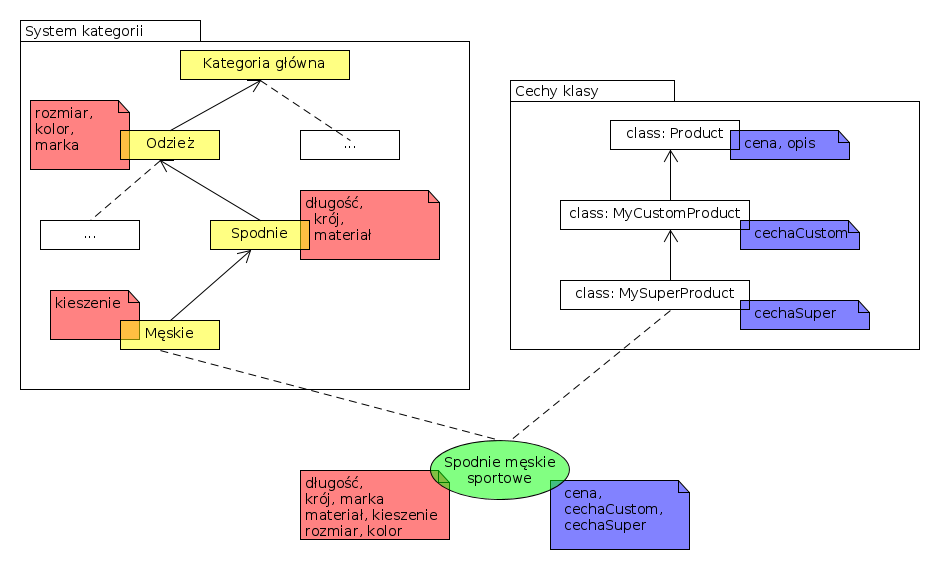
\includegraphics[scale=0.3]{cechyProd.png}
		\end{center}
		\caption{{\color{black}Diagram przykładowy pochodzenia atrybutów produktu}} \label{cechyProd}
	\end{figure}
\end{frame}

\begin{frame}{[TODO] System uprawnień}{Jak będzie działać system uprawnień w panelu administracyjnymm}
\begin{itemize}
	\item<1-> użytkownik administracyjny będzie miał kolekcję uprawnień
	\item<2-> struktura systemu uprawnień będzie podobna do struktury kategorii, uprawnienia będą mogły po sobie dzidziczyć
	\item<3-> AdminMenuGroup i AdminMenuItem będą miały kolekcje encji 'uprawnienie', podczas \textit{renderu} menu, będą brane pod uwagę, względem tego, kto jest aktualnie zalogowany
\end{itemize}
\end{frame}

\begin{frame}{Klasyczne funkcjonalności}{Inne (niekoniecznie ciekawe) funkcjonalności, które muszą być w sklepie}
\begin{itemize}
	\item<1-> koszyk
	\item<1-> logowanie jako uzytkownik sklepu 
	\item<1-> możliwość dokonania zakupu
	\item<1-> zarządzanie zamówieniami/użytkownikami/adresami 
	\item<1-> i pare innych... 
\end{itemize}
\end{frame}

\subsection{Mechanizm indeksująco-wyszukujący}

\begin{frame}{Mechanizm indeksująco-wyszukujący}{Integracja płaskiej bazy no-sql z bazą relacyjną}
\begin{itemize}
	\item<1-> do zapytań związanych z katalogiem produktowym użyto serwer Apache Solr 7.5 oparty na silniku Lucene
	\item<2-> Solr umożliwia dobrą i wszechstronną analizę danych tekstowych, podświetlanie, podpowiadanie i facetowanie. 
	\item<3-> (TODO) co jakiś czas uruchamiany jest Job w systemie, który synchronizuje bazę relacyjną z Solrem (na razie za każdym requestem)
	\item<4-> Indeksacja to wydobycie atrybutów wyszukiwalnych i facetowalnych z produktu, zapakowanie w dokumenty i wysłane na serwer Solr - wyciągnięcie atrybutów pokazuje rysunek \ref{cechyProd}
	
\end{itemize}
\end{frame}

\begin{frame}{Indeksacja atrybutów produktu}{Jak zachowano elastyczność?}
\begin{itemize}
	\item<1-> atrybuty niepochodzące z systemu klasyfikacyjnego są również indeksowane
	\item<2-> pola w klasach rozszerzających \texttt{Product} (np. \texttt{MyProduct extends Product}) są również możliwe do zaindeksowania, wystarczy że z poziomu panelu administracyjnego dodamy do tabeli SearchField nazwę pola, reszta zrobi się sama
\end{itemize}
\end{frame}

\part{Przykłady działania}
 
\begin{frame}{Indeksacja atrybutów produktu}{Jak zachowano elastyczność?}
\begin{itemize}
	\item<1-> atrybuty niepochodzące z systemu klasyfikacyjnego są również indeksowane
	\item<2-> pola w klasach rozszerzających \texttt{Product} (np. \texttt{MyProduct extends Product}) są również możliwe do zaindeksowania, wystarczy że z poziomu panelu administracyjnego dodamy do tabeli SearchField nazwę pola, reszta zrobi się sama
\end{itemize}
\end{frame}
%%%%%%%%%%%%%%%%%%%%%%%
%%%%% Slajd  %%%%%%%%%%
%%%%%%%%%%%%%%%%%%%%%%%
\begin{frame}{Dynamiczny panel administracyjny}{Panel administracyjny, który umożliwi zarządzanie wszystkimi encjami w systemie}
\begin{exampleblock}{Przykład}
przykład 1
\end{exampleblock}
%%%%%%%%%%%%%%%%%%%
\begin{definition}
Dystrybucją \LaTeX a nazywamy \ldots
\end{definition}
%%%%%%%%%%%%%%%%%%%
\begin{theorem}[Pitagorasa]
$a^2+b^2=c^2$
\end{theorem}
%%%%%%%%%%%%%%%%%%%
\pause %To, co poniżej ma być umieszczone w kolejnej warstwie oraz wszystkich następnych
\begin{proof}
Treść dowodu
\end{proof}
%Jeśli rysunek1.pdf jest wielostronicowym rysunkiem (np. utworzonym za pomocą programu 'Ipe'), parametr 'page=nr' powoduje wyświetlenie strony o podanym numerze
%\includegraphics<1>[page=1,scale=0.5,angle=-90]{rysunek1.pdf}
%\includegraphics<2>[page=2,scale=0.5,angle=-90]{rysunek1.pdf}
\end{frame}

%%%%%%%%%%%%%%%%%%%%%%%%%%%%%%%%%%%
%%%%% Tytuł podrozdziału %%%%%%%%%%
%%%%%%%%%%%%%%%%%%%%%%%%%%%%%%%%%%%
\subsection{Zagadnienie 1.2}

%%%%%%%%%%%%%%%%%%%%%%%
%%%%% Slajd  %%%%%%%%%%
%%%%%%%%%%%%%%%%%%%%%%%
\begin{frame}{Tytuł slajdu 3}
treść slajdu 3
%\scalebox{0.5}{ \input{rysunek2.pdftex_t} }  
\end{frame}

%%%%%%%%%%%%%%%%%%%%%%%
%%%%% Slajd  %%%%%%%%%%
%%%%%%%%%%%%%%%%%%%%%%%
\begin{frame}{Tekst w wielu kolumnach}
% Otoczenie 'columns' pozwala na składanie tekstu w wielu kolumnach.
% Poszczególne kolumny definiuje się za pomocą komendy 'column'
\begin{columns}
%Utwórz kolumnę o rozmiarze: 60% szerokości tekstu 
\column{0.6\textwidth}
\begin{description}
\item[Pojęcie 1] \pauza wyjaśnienie pojęcia 1
\item[Pojęcie 2] \pauza wyjaśnienie pojęcia 2
\end{description}

%Utwórz kolumnę o rozmiarze: 40% szerokości tekstu 
\column{0.4\textwidth}
\structure{Treść prawej kolumny}
\begin{enumerate}
\item pozycja 1
\item pozycja 2
\end{enumerate}
\end{columns}
\end{frame}

%%%%%%%%%%%%%%%%%%%%%%%%%%%%%%%%
%%%%% Tytuł rozdziału %%%%%%%%%%
%%%%%%%%%%%%%%%%%%%%%%%%%%%%%%%%
\section{Zagadnienie 2}

%%%%%%%%%%%%%%%%%%%%%%%
%%%%% Slajd  %%%%%%%%%%
%%%%%%%%%%%%%%%%%%%%%%%
\begin{frame}{Tytuł slajdu 5}
%Określamy kolor wierszy parzystych i nieparzystych tabeli w oparciu o aktualną kolorystykę bloku
\rowcolors{2}{block title.bg}{block body.bg}
\begin{table}
\begin{tabular}{|r|p{4cm}|l|}\hline
\textbf{Kol$_{1}$} &\textbf{Kol$_{2}$} &\textbf{Kol$_{3}$}\\
\hline
\hline
& & \\
& & \\
& & \\
& & \\
& & \\
& & \\
\hline
\end{tabular}
\end{table}
\end{frame}

%%%%%%%%%%%%%%%%%%%%%%%
%%%%% Slajd  %%%%%%%%%%
%%%%%%%%%%%%%%%%%%%%%%%
\part{Literatura}
% Aby tytuł rozdziału, tu  'Literatura', nie pojawił się na slajdzie z planem prezentacji, 
% należy użyć rozkazu \section* (gwiazdka po słowie 'section') 
\section*{Literatura}
\begin{frame}[allowframebreaks]{Literatura}
%Parametr 'allowframebreaks' oznacza, że jeżeli treść nie mieści się na jednym slajdzie, to LaTeX powinien utworzyć dodatkowe slajdy
\begin{thebibliography}{}
% Komenda  '\setbeamertemplate{bibliography item}[article]' oznacza, że poszczególne pozycje są artykułami i~w~związku z~tym każda z~pozycji będzie poprzedzona ikoną artykułu
% Domyślnie, poszczególne pozycje są poprzedzone ikoną artykułu, dlatego tego rozkazu nie musimy tu umieszczać
% \setbeamertemplate{bibliography item}[article]
    \bibitem{poz1}
      Imię i~nazwisko autora 
      \newblock
      Tytuł artykułu 
      \newblock 
      pozostałe informacje (nazwa czasopisma, numer, \ldots) 
      \newblock
      informacje dodatkowe (adres strony WWW, \ldots)
    \bibitem{poz2}
      Imię i~nazwisko autora 
      \newblock 
      Tytuł artykułu 
      \newblock
      pozostałe informacje (nazwa czasopisma, numer, \ldots)
      \newblock informacje dodatkowe (adres strony WWW, \ldots)
    
  %Komenda '\setbeamertemplate{bibliography item}[book] oznacza, że poszczególne pozycje są książkami i~w~związku z~tym każda z~pozycji będzie poprzedzona ikoną książki
  \setbeamertemplate{bibliography item}[book]
    \bibitem{poz3} 
      Imię i~nazwisko autora
      \newblock
      Tytuł książki
      \newblock
      pozostałe informacje (rok wydania, wydawca, \ldots)
      \newblock informacje dodatkowe (adres strony WWW, \ldots)
    \bibitem{poz4} 
      Imię i~nazwisko autora
      \newblock 
      Tytuł książki
      \newblock
      pozostałe informacje (rok wydania, wydawca, \ldots)
      \newblock informacje dodatkowe (adres strony WWW, \ldots)
    
  \setbeamertemplate{bibliography item}[online]
    \bibitem{poz5}
      Wujek Google
      \newblock
      \url{http://www.google.pl/}
\end{thebibliography}
%%%%%%%%%%%%%%%%%%%%%%%%%%%%%%%%%%%%%%%%%%%%%%%%%%%%%%%%%%%%%%%%%%%%%%%%%%
% Jeśli literaturę mamy w pliku 'literatura.bib' i chcemy używać Bibtex-a,
% należy odkomentować poniższe linie oraz usunąć całe 'thebibliography'
%%%%%%%%%%%%%%%%%%%%%%%%%%%%%%%%%%%%%%%%%%%%%%%%%%%%%%%%%%%%%%%%%%%%%%%%%%
%\bibliography{literatura}
%\bibliographystyle{plplain}
%\nocite{poz1}
%\nocite{poz2}
\end{frame}
\end{document}
